\documentclass[letter,11pt]{article}
\usepackage[spanish, activeacute]{babel}
\usepackage{amsfonts}
\usepackage{amsmath,amsfonts,amssymb}
\usepackage{fancyhdr}
\usepackage{fancyvrb}
\usepackage{xy}
\usepackage{graphicx}
\usepackage{latexsym,amsfonts}
\usepackage{enumerate}
\usepackage{multirow}
\usepackage{multicol}
\usepackage{hyperref}
\usepackage{longtable}
\usepackage{hyperref}
\hypersetup{
    colorlinks=true,       % false: boxed links; true: colored links
    linkcolor=red,          % color of internal links (change box color with linkbordercolor)
}
\textwidth 160mm
\textheight 235mm
\oddsidemargin 0.7cm
\topmargin -1cm

\usepackage[numbered,framed]{matlab-prettifier}
\lstMakeShortInline"
\lstset{
  style              = Matlab-editor,
  escapechar         = ",
  mlshowsectionrules = true,
}

\setlength{\oddsidemargin}{-0.5cm}
\setlength{\evensidemargin}{0cm} \setlength{\textwidth}{17.5cm}
\setlength{\textheight}{24cm} \setlength{\topmargin}{-1.7cm}

\title{lab03 521230 2018-1}

\font\bff=cmbx10 at 10truept
\font\lg=cmdunh10 at 10truept
\font\bl=cmss10 at 10truept

\newcommand\R{\mathbb{R}}
\newcommand\IN{\mathbb{N}}
\newcommand\Z{\mathbb{Z}}
\newcommand\bsi{{\mbox{\boldmath $\sigma$}}}
\newcommand\bta{{\mbox{\boldmath $\tau$}}}
\newcommand\bet{{\mbox{\boldmath $\eta$}}}
\newcommand\bga{{\mbox{\boldmath $\gamma$}}}
\newcommand\bze{{\mbox{\boldmath $\zeta$}}}
\newcommand{\dis}{\displaystyle}

\renewcommand\u{\mathbf{u}}
\newcommand\bv{\mathbf{v}}
\newcommand\0{\mathbf{0}}

\newcommand{\matlab}{{\sc Matlab} }

\newcommand{\header}{\noindent%
{\lg UNIVERSIDAD DE CONCEPCI\'ON}\hfill
\vskip-4truept
\noindent{\bff FACULTAD DE CIENCIAS}\hfill
\vskip-4truept
\noindent{\bff F\'ISICAS Y MATEM\'ATICAS}\hfill
\vskip-4truept
\noindent{\bl DEPARTAMENTO DE INGENIER\'IA MATEM\'ATICA}\hfill
\vskip4truept\hrule\hrule\vskip4truept
\par
}

\begin{document}
\header
\vspace{0.7cm}
\begin{center}
\textbf{\small C\'alculo Num\'erico (521230) - Laboratorio 3}\\
\vspace{0.1cm}
\textbf{\Large ECUACIONES NO LINEALES EN MATLAB}
\vspace{0.7cm}
\end{center}
En la teor\'ia hemos visto cuatro m\'etodos para la resoluci\'on de ecuaciones no lineales, por un lado: de la bisecci\'on, Newton Raphson y de la secante, los cuales est\'an orientados a resolver ecuaciones de una variable. Y finalmente el m\'etodo de Newton, que consiste en una generalizaci\'on del m\'etodo de Newton Raphson, que permite resolver sistemas de ecuaciones no lineales.

\section{M\'etodo de la bisecci\'on.}
	Descargue el programa
     \href{ftp://ftp.ing-mat.udec.cl/pub/ing-mat/asignaturas/521230/ejercicios/2018-1/biseccion.m}{biseccion.m}, este programa consuste en un rutero que implementa el m\'etodo de la bisecci\'on para resolver una ecuaci\'on no lineal en particular.
     
    Considerando este programa
\begin{enumerate}
	\item Descargue el programa mencionado y ejec\'utelo. \textquestiondown Qu\'e observa en la ejecuci\'on de este programa?.
    \item Comente las l\'ineas de c\'odigo en los espacios disponibles. Usando una frase que describa brevemente el objetivo de cada l\'inea del programa.
    \item Cree una variable que almacene la cantidad de pasos realizados en el algoritmo implementado en el programa.
    \item Modifique el criterio de detenci\'on para que sea mediante una tolerancia de $10^{-8}$ \'o $350$ iteraciones.
    \item A partir del programa cree una funci\'on que tenga como entradas los extremos iniciales del m\'etodo y que retorne la ra\'iz calculada con el criterio de detenci\'on anterior. 
    \item Use esta funci\'on para calcular todas las ra\'ices negativas que se observan en la gr\'afica del programa.
\end{enumerate}

Use el programa estudiado en los pasos anteriores para encontrar al menos dos ra\'ices de las ecuaciones no lineales, si existen.
\begin{multicols}{3}
\begin{enumerate}
	\item $x^3+2x=-8$
	\item $x^2/\cos(x)=x$,
    \item $2x^2 +\cos(x) =x$,
    \item $\frac{\sen(x)}{x^2+1}=0$,
    \item $\frac{e^{x^2+1}}{e^{-x}}=x$,
    \item $\frac{\tan(x)}{1+x}=2x+1$,
\end{enumerate}
\end{multicols}

\section{M\'etodo de Newton-Raphson.}
Descargue el programa
    \href{ftp://ftp.ing-mat.udec.cl/pub/ing-mat/asignaturas/521230/ejercicios/2018-1/newtonraphson.m}{newtonraphson.m}, este programa consiste en un rutero que implementa el m\'etodo de Newton-Raphson para resolver una ecuaci\'on no lineal en particular.
       
    Considerando este programa
\begin{enumerate}
	\item Descargue el programa mencionado y ejec\'utelo. \textquestiondown Qu\'e observa en la ejecuci\'on de este programa?.
    \item Comente las l\'ineas de c\'odigo en los espacios disponibles. Usando una frase que describa brevemente el objetivo de cada l\'inea del programa.
    \item Modifique el programa para que comienze con los siguientes puntos iniciales
    $$
    1.5, \quad 3.0, \quad 2.35, \quad 1.
    $$
    \textquestiondown Qu\'e observa en la ejecuci\'on del programa considerando estos puntos iniciales?.
   \item Modifique el criterio de detenci\'on para que sea mediante una tolerancia de $10^{-4}$ 
   programa.
\end{enumerate}

Use el programa estudiado en los pasos anteriores para encontrar al menos dos r\'aices de las ecuaciones no lineales, si existen.
\begin{multicols}{3}
\begin{enumerate}
	\item $\cos(x^2+1)=1$,
    \item $2x^3-\sen(x^2+1)=x$,
    \item $e^{\cos(x+1)}=1$.
\end{enumerate}
\end{multicols}
\textbf{Observaci\'on:} En este caso debe calcular anal\'iticamente la derivada de cada funci\'on.

\section{M\'etodo de la secante.}
Usando lo desarrollado con los programas anteriores, construya un rutero de \matlab  que permita resolver la ecuaci\'on no lineal
$$
\frac{\cos(x^2+2x+1)}{x^2+1}=x
$$
considerando como puntos iniciales $x_0=2.5$ y $x_1=1.5$ mediante el m\'etodo de la secante. Para esto se sugiere:
\begin{enumerate}
\item Crear una funci\'on tipo inline que represente a la funci\'on asociada a la ecuaci\'on no lineal.
\item Grafique esta funci\'on.
\item Definir los puntos iniciales del algoritmo.
\item Para poder observar el comportamiento del algoritmo, grafique los puntos iniciales en la gr\'afica de esta funci\'on.
\item Programe un ciclo iterativo que permita hacer los c\'alculos de cada paso. Recuerde que debe considerar alg\'un criterio de detenci\'on.
\item Dentro de este ciclo iterativo, realice el c\'alculo del siguiente punto del m\'etodo.
\item Dentro de este ciclo iterativo, grafique en la funci\'on el siguiente punto calculado.
\end{enumerate}

Una vez que tenga implementado este programa, proponga puntos iniciales m\'as adecuados para construir la aproximaci\'on a la soluci\'on buscada.

\section{Ejercicios.}
\begin{enumerate}

\item Mediante alg\'un m\'etodo num\'erico adecuado encuentre soluciones de los siguientes problemas.
\begin{enumerate}
	\item El ancho de un rect\'angulo es $2[cm]$ mas largo que tres veces su alto. Si el \'area del rect\'angulo es $56[cm^2]$, \textquestiondown Cuales son las dimensiones del rect\'angulo?. 
    \item Use el m\'etodo de Newton-Raphson para encontrar el menor valor de $x$ que satisface
    $$
    0.7=\frac{1}{2}\left(1+\sen(x)e^{-\frac{x}{2\pi}}\right)
    $$
	\item En mec\'anica y f\'isica son de inter\'es encontrar puntos fijos de funciones no lineales. Un punto fijo $x_0$ de una funci\'on $f$, es un punto en el dominio de la funci\'on donde se satisface
    $$
    f(x_0)=x_0.
    $$
    Por ejemplo, la funci\'on $f(x)=x^2+3x+1$ tiene como punto fijo $x=-1$. Calcule puntos fjos de las funciones
    \begin{multicols}{3}
    \begin{enumerate}
    	\item $f(x)=0.9x^2-1.7x-2.5$,
        \item $g(x)=\sen(\sqrt{x})-x$,
        \item $h(x)=2\sen(x)-\frac{x^2}{8}$,
    \end{enumerate}
    \end{multicols}
    
\item Con los programas analizados y construidos en las secciones anteriores, construya un programa que genera una celda que tenga los siguientes datos:
\begin{center}
\begin{tabular}{||c|c|c|c|}
\hline
N. de iteraci\'on & Error Bisecci\'on & Error Newton-Raphson & Error Secante \\
\hline
1 	& & & \\
\hline
2 	& & & \\
\hline
$\vdots$ 	& & & \\
\hline
\end{tabular}
\end{center}
considerando la b\'usqueda de soluciones de la ecuaci\'on
$$
(x^3+2x+1)\, \cos(x^3+1)=2
$$
con puntos iniciales $x_0=2.2$ para el m\'etodo de Newton-Raphson y $x_a=2$,$x_b=2.2$ para el m\'etodo de la bisecci\'on y la secante.
    
\end{enumerate}
\end{enumerate}

\section{El m\'etodo de Newton}
Cuando nos enfrentamos a un sistema de ecuaciones lineales, ninguno de los m\'etodos estudiados anteriomente es adecuado. Sin embargo, se puede considerar una generalizaci\'on del m\'etodo de Newton-Raphson. Similar a lo visto anteriormente, buscar una soluci\'on del sistema
$$
\begin{array}{c|}
\cos(x)-y=-2x\\
y-x^2=0 \\
\hline
\end{array}
$$
puede ser planteado como encontrar una preim\'agen del vector nulo para el campo vectorial
$$
f(x,y)=(\cos(x)-y+2x,\,y-x.^2).
$$
Seg\'un lo visto en la teor\'ia, usando una aplicaci\'on lineal afin, se construye una sucesi\'on de aproximaciones a partir de una preim\'agen $x_0$ para $f$
$$
x_{k+1}=x_k+Df(x_k)^{-1} f(x_k), \quad \forall k\in\{0,1,\cdots,n\}
$$
que se espera convergan a la ra\'iz buscada. Siguiendo el ejemplo anterior,
$$
\begin{bmatrix}
x_{k+1}\\y_{k+1}
\end{bmatrix}
=
\begin{bmatrix}
x_{k}\\y_{k}
\end{bmatrix}
+
\left.\begin{bmatrix}
2x_{k} -y_{k} \,sen(x_{k} y_{k}) & - x_{k}\,\sen(x_{k} y_{k}) \\
2 & 1
\end{bmatrix} \right.^{-1}
\begin{bmatrix}
 x_{k}^2+\cos(x_{k} y_{k})-1\\
2x_{k}+y_{k}
\end{bmatrix}
$$
En la ejecuci\'on de este algoritmo podemos considerar como criterio de detenci\'on las mismas ideas vistas anteriormente:
\begin{enumerate}
\item Cantidad de iteraciones.

	En este caso, se cuentan la cantidad de veces que se ha calcula una nueva aproximaci\'on de la ra\'iz. Cuando se llegue a un valor m\'aximo, se termina la ejecuci\'on del programa y se considera como soluci\'on num\'erica la \'ultima obtenida.

\item Distancia entre las ra\'ices sucesivas.

En este caso se debe proveer al m\'etodo una tolerancia. As\'i, cada vez que se realize el c\'alculo de una nueva aproximaci\'on a la soluci\'on $x_{k+1}$, se debe chequear que la magnitud
$$
||x_{k+1}-x_{k}||
$$
siga siendo mayor que la tolerancia. Si el resultado es menor, entonces se termina el m\'etodo y se considera la \'ultima calculada como soluci\'on.

\item Cercan\'ia al cero a trav\'es de la funci\'on.

Similarmente al caso anterior, se considera una tolerancia fija y se ejecuta el m\'etodo mientras
$$
\|f(x_k)\|
$$
siga siendo menor que la tolerancia. Si en alg\'un paso esta norma es menor que la tolerancia, se detiene la ejecuci\'on y se retorna como soluci\'on num\'erica la \'ultima ra\'iz aproximada.

\textbf{Observaci\'on:} Gracias a la equivalencia de normas, da lo mismo cual norma se considere en los criterios de detenci\'on b) y c).

\end{enumerate}

\subsection{Ejercicios}
Descargue y ejecute el programa
    \href{ftp://ftp.ing-mat.udec.cl/pub/ing-mat/asignaturas/521230/ejercicios/2018-1/newton.m}{newton.m}, este programa consiste en un rutero que implementa el m\'etodo de Newton para resolver el sistema de ecuaciones no lineales anterior. Considerando este rutero:
    
    \begin{enumerate}
    \item Modifique el rutero descargado para considerar como criterio de detenci\'on un n\'umero m\'aximo de 150 iteraciones \'o una tolerancia de $10^{-8}$ en las formas de detenci\'on descritas anteriomente.
    \item Modifique la ra\'iz inicial del problema para calcular obtener soluciones num\'ericas de las restantes ra\'ices de este problema.
    \item Modifique el rutero descargado para resolver los problemas de ecuaciones no lineales
    \begin{multicols}{3}
    \begin{enumerate}
    \item $\begin{array}{c|}
		   \cos(xy)*x=1\\
           \sen(xy)*y=0\\
           \hline
           \end{array}$
           
      \item $\begin{array}{c|}
		   2*x^2+y^2=1\\
           3*x+y^2=2\\
           \hline
           \end{array}$
           
       \item $\begin{array}{c|}
		   x+yz=0\\
           y-x^2=0\\
           \cos(z)=0\\
           \hline
           \end{array}$
    \end{enumerate}
    \end{multicols}
    
    \item Usando el m\'etodo de Newton, encuentre un punto cr\'itico de la funci\'on
    $$
    f(x,y)=2x^2y^2+x^2y-2x-y^2.
    $$
    
    \item Encuentre las intersecciones de las elipse y par\'abolas de ecuaciones
    $$
    2x^2+y^2=1 , \quad y=-2x^2.
    $$
    \end{enumerate}
    

\newpage
\section{Utilizaci\'on de funciones propietarias de \matlab}
Los m\'etodos num\'ericos programados y estudiados anteriomente, est\'an disponibles entre las funciones propias de \matlab \texttt{fzero()} y \texttt{fsolve()}. Los siguientes ejemplos muestran el uso de estas funciones y sus distintas variables.

\subsection{Un problema de enfriamiento no lineal}
El Sr.\ D fue encontrado muerto en su oficina a las 20:00 hrs del 22 de octubre de 2012, la
		temperatura de su cuerpo era de $32.2[^\circ C]$. Una hora despu\'es,
		\'esta hab\'{\i}a descendido a $29.4[^\circ C]$.

		El Capit\'an F cree que M es el asesino. Sin embargo, M dice
		tener una coartada: fue entrevistado entre 18:40 y 19:15 por el periodista J. Efectivamente, en la recepci\'on
		del edificio donde se realiz\'o la entrevista se registr\'o la llegada de M a las 18:35 y su salida
		a las 19:20. ?`Pudo M ser el asesino? Debemos determinar la hora de la muerte del Sr. D.

		Supongamos que $T(t)$ denota la temperatura del cuerpo del Sr. D en el instante de tiempo $t$.
		Con los datos anteriores sabemos que
		$T(20) = 32.2$, $T(21) = 29.4$. Adem\'as, seg\'un la ley de Newton,
		\[
			\frac{\mbox{d}T}{\mbox{d}t} = -\kappa\left(T(t) - T_{\mbox{ambiente}}(t)\right),
		\]
		donde $\kappa$ es una constante y $T_{\mbox{ambiente}}(t)$ es la temperatura ambiente en el tiempo $t$.
		De la temperatura de la oficina del Sr. D (lugar d\'onde fue encontrado su cuerpo) sabemos que
		a las 16:00 hrs era de 20 grados, sin embargo a esa hora se report\'o un da\~no
		en el aire acondicionado de la misma y la temperatura comenz\'o a ascender
		a partir de ese momento a raz\'on de $0.5$ grados por hora, es decir
		podemos tomar
		\[
			T_{\mbox{ambiente}}(t) = \begin{cases}
										20, & t \le 16,\\
										20 + \frac 1 2 (t-16), & t > 16
			                      \end{cases}
		\]

		Resolviendo el problema de valores iniciales (v\'alido s\'olo para $t \ge 16$),
		\[
			\frac{\mbox{d}T}{\mbox{d}t} = -\kappa\left(T(t) - 20 - \frac 1 2(t-16)\right),\quad T(20) = 32.2
		\]
		se tiene
		\[
			T(t) = \left(10.2 + \frac{1}{2\kappa}\right)e^{-\kappa(t-20)} + \frac{t + 24}{2} - \frac{1}{2\kappa},\quad t \ge 16.
		\]

		Con esta expresi\'on para $T$ y sabiendo que $T(21) = 29.4$, determine la hora de la muerte del Sr. D, es decir,
		determine el momento de tiempo $16 < t_* < 20$ en que la temperatura
		del cuerpo del Sr. D era $36.5$ grados.		

		Debemos resolver 2 problemas no lineales: el primero es determinar $\kappa$ de modo que $T(21) = 29.4$ y el segundo es,
		una vez conocido $\kappa$, determinar $t_*$.

		Sea
		\[
			F(\kappa) = T(21) - 29.4,
		\]
		\begin{enumerate}
			\item \label{funcionF} Escriba una funci\'on \matlab\, que dado $\kappa \in \R$ (par\'ametro de entrada
				a la funci\'on), calcule $F(\kappa)$. Esta funci\'on debe estar
				escrita de modo que, en caso que el par\'ametro de entrada sea un vector, ella
				retorne un vector con los valores de $F$ en cada uno de los puntos especificados
				en el vector de entrada.

			\item \label{encontrarkappa} Escriba un rutero \matlab\, que haga lo siguiente:
				
				\begin{enumerate}
					\item eval\'ue $F$ en 100 puntos distintos del intervalo $[0.1,\,0.5]$. Haga un gr\'afico de
						la funci\'on y observe que ella tiene un cero en el intervalo considerado. Con la ayuda del comando \verb+grid on+ indique una aproximaci\'on inicial de la ra\'iz de esta funci\'on.

					\item Llame a la funci\'on \matlab\, \verb+fzero+
						para obtener una aproximaci\'on al cero de $F$ en $[0.1,\,0.5]$.
						Ello lo logra escribiendo {\bf una} de las siguientes l\'{\i}neas en su programa, tenga
						presente que debe sustituir \verb+Fkappa+ por el nombre de la funci\'on escrita por usted antes.

						\medskip
							
						\begin{Verbatim}[gobble=6,frame=single,numbers=left]
						kappa = fzero('Fkappa',0.2,optimset('TolX',1e-10))

						kappa = fzero('Fkappa',[0.1,0.5],optimset('TolX',1e-10))
						\end{Verbatim}
						
						\medskip

						Para entender los llamados anteriores a \verb+fzero+,
						lea la siguiente explicaci\'on acerca
						de este comando: \verb+fzero+ es una funci\'on \matlab\, para la aproxi\-ma\-ci\'on
						de ra\'{\i}ces de funciones reales basada en una combinaci\'on del
						m\'etodo de bisecci\'on con el m\'etodo de la secante y otras t\'ecnicas.
						{\em El primer par\'ametro
						de entrada} a \verb+fzero+ es la funci\'on cuya ra\'{\i}z quiere aproximarse.
						{\em El segundo par\'ametro de entrada} puede ser un n\'umero real
						o un vector de 2 componentes. Si es un n\'umero real, es considerado
						como una aproximaci\'on inicial al cero de la funci\'on. Si es un vector
						de 2 componentes, representa el intervalo inicial donde buscar el cero
						de la funci\'on (debe cumplir con las exigencias del m\'etodo de bisecci\'on). En ambos casos, estos par\'ametros pueden ser estimados mediante la gr\'afica de la funci\'on.
						{\em Los siguientes pa\-r\'a\-me\-tros de entrada} son opcionales. En este caso, especificamos
						que la precisi\'on con que quiere calcularse la aproximaci\'on al cero de $F$ debe
						ser $10^{-10}$ (\verb+'TolX',1e-10+). La forma en que
						procede \verb+fzero+ en cada caso puede leerla escribiendo
						\verb+help fzero+ en la ventana de comandos de \matlab.
						
						\medskip

						Escriba el valor de $\kappa$ obtenido.

						\medskip

						\def\arraystretch{1.5}
						\begin{center}
							\begin{tabular}{|p{.8in}|p{4in}|}
								\hline $\kappa$ & \\
								\hline
						\end{tabular}\end{center}
						\medskip

\textbf{Nota 1:} Puede definir una funci\'on mediante un programa \verb"funcion.m" o mediante el comando \verb"inline", por ejemplo, para $f(x)=x^2-1$.

						\medskip
							
						\begin{Verbatim}[gobble=6,frame=single,numbers=left]
						f=inline('x.^2-1')          % Define una funcion en terminos de x 
						f(1)                       % Evalua la funcion anterior en x=1
						feval(f,1)                 % Identico a lo anterior
						\end{Verbatim}
						
						\medskip


\textbf{Nota 2:} Si tiene una funci\'on con muchas entradas pero solo una de ellas es una variable, puede utilizar \verb"fzero" con el comando \verb"@(x)". Por ejemplo.

						\medskip
							
						\begin{Verbatim}[gobble=6,frame=single,numbers=left]
						f=inline('x.^2-y.^2');

						xo=fzero(@(x)f(x,4),1.5)
						yo=fzero(@(y)f(4,y),1.5)
						\end{Verbatim}
						
						\medskip



				\end{enumerate}

			\item Escriba ahora una funci\'on que eval\'ue a $T(t)-36.5$ tomando $\kappa$ igual
				al valor obtenido antes.


			\item Proceda de manera similar a como lo hizo en 1.2, pero ahora para determinar
				el valor de $t_* \in (16,\,20)$ en el cual la temperatura del Sr. D era de
				36.5. ?`A qu\'e hora fue asesinado el Sr. D?
				
					\medskip
							
					\begin{Verbatim}[gobble=6,frame=single]
					
					
					
					
					\end{Verbatim}
					
					\medskip
				
%				\newpage
					\noindent ?`Pudo M asesinar a D?
				
					\medskip
							
					\begin{Verbatim}[gobble=6,frame=single]
					
					
					
					
					\end{Verbatim}
					
					\medskip

\subsection{Un problema de asignaci\'on}

Juan y Beatriz trabajan en una empresa pesquera que procesa $200[Kg]$ diarios de salm\'on. Este Lunes Juan empez\'o a trabajar a las 8:00AM y alcanz\'o a hacer $100[Kg]$ justo cuando Beatriz lleg\'o. Luego Beatriz sigui\'o trabajando y termin\'o el trabajo a las 8:50AM. El martes ambos empezaron el trabajo a las 8:00AM y terminaron a las 8:24AM. El mi\'ercoles Beatriz estaba enferma. Si Juan es el trabajador m\'as r\'apido, \textquestiondown Cuanto tiempo le tomar\'a a Juan completar los $200[Kg]$ de salm\'on a el s\'olo?.

\begin{enumerate}
\item En este problema se identifica que las inc\'ognitas:
\begin{enumerate}
\item $J$: rapidez de trabajo de Juan medida en $[kg/min]$.
\item $B$: rapidez de trabajo de Beatiz medida en $[kg/min]$.
\item $t_0$:  tiempo del d\'ia Lunes en los que Juan trabaj\'o solo medido en $[min]$.
\end{enumerate}
\item Considerando estas variables, del enunciado sigue el siguiente sistema de ecuaciones no lineales
$$
\begin{array}{lr|}
J\cdot t_0	&=100\\
B\cdot(50-t_0)	&=100\\
J\cdot 24 + B\cdot 24 &=200\\
\hline
\end{array}
$$
\item Siguiente este sistema de ecuaciones, estamos interesados en encontrar una ra\'iz al campo vectorial
$$
f_p(J,B,t_0)=(J\cdot t_0-100, B\cdot(50-t_0)-100, 24J+24B-200).
$$
Para hacer esto, cree un fichero tipo \texttt{function} que permita evaluar, mediante vectores, este campo vectorial. Este archivo debe contener instrucciones similares a
\begin{lstlisting}
function y=fp(x)
	y(1)=x(1)*x(3)-100;
	y(2)=x(2)*(50-x(3))-100;
	y(3)=24*x(1)+24*x(2)-200;
\end{lstlisting}
Para verificar que esta funci\'on est\'a bien ingresada eval\'uela en $[0,0,0]$. \textquestiondown Cuanto debe retornar esta funci\'on?.

\item Las siguientes instrucciones permiten resolver usando la funci\'on \texttt{fsolve} de  \matlab
\begin{lstlisting}
x0 = [0,0];
x = fsolve(@fp,x0)
\end{lstlisting}
para verificar que la soluci\'on obtenida es correcta, observe la evaluaci\'on de la funci\'on $f_p$ en la soluci\'on num\'erica calculada.
\item ¿Cuanto tiempo le tomar\'a a Juan completar los $200[Kg]$ s\'olo?.
\end{enumerate}

\end{enumerate}
	
\subsection{Ejercicios}
Usando las funciones privativas de \matlab \texttt{fzero()} o \texttt{fsolve()} seg\'un corresponda, resuelva los siguientes problemas de ecuaciones no lineales.

\begin{enumerate}
\item Encuentre el largo de los catetos de un tri\'angulo rect\'angulo cuya hipotenusa mide $\sqrt{15}[cm]$ y su \'area es $3[cm]^2$.
\item La etiqueta de una televisi\'on pequeña dice que tiene $5''$ de diagonal y una superficie de 12 pulgadas cuadradas. \textquestiondown Cual es el largo y ancho de la pantalla?.
\item Vicente tiene un plano para construir una casa con siete frontones. El plano pide que en cada front\'on vaya una ventilaci\'on con forma de tri\'angulo Isoceles. Debido a la inclinaci\'on del techo, la raz\'on entre la altura y la base de cada tri\'angulo debe ser 1 es a 4. Si las ventilaciones deben proveer un total de $3500[cm^2]$, \textquestiondown Cuanto deber\'ia medir la base y la altura de cada tri\'angulo?.
\begin{center}
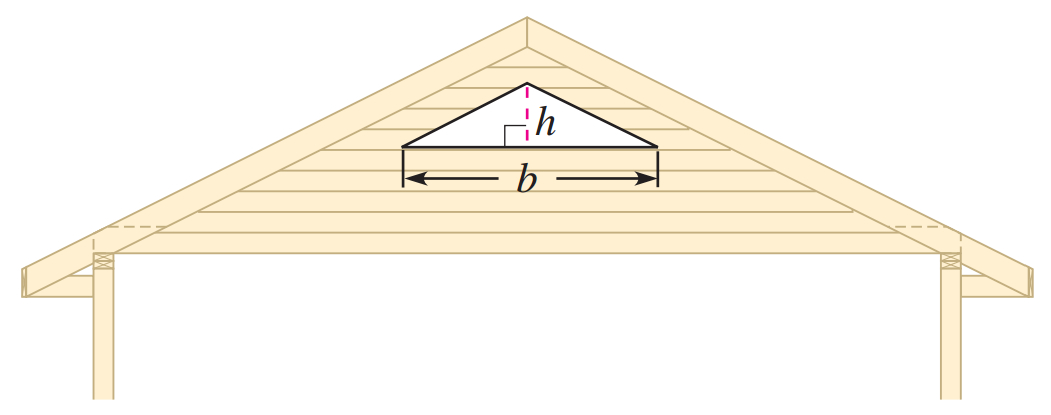
\includegraphics[width=0.5\textwidth]{./p1.jpg}
\end{center}
\item Una bomba $A$ puede llenar o vaciar un tanque en el mismo tiempo. Si las bombas $A$ y $B$ trabajan juntas, el tanque se puede llenar en $6$ horas. Al equivocarse los operadores pusieron a la bomba $A$ vaciando el tanque y a la bomba $B$ llen\'andolo, tom\'o $12$ horas llenar el tanque. \textquestiondown Cuanto tiempo le toma a cada una de estas bombas llenar el tanque solas?.

 \item Daniela ordena o desordenada su casa la misma velocidad. Cuando Daniela est\'a ordenando con su madre, logran ordenar una casa totalmente desordenada en $6$ horas. Si Daniela no ayuda a su madre, a ella le toma $9$ horas ordenar la casa mientras Daniela est\'a continuamente desordenando. \textquestiondown Cuanto tiempo le toma a la madre de Daniela ordenar la casa, si Daniela es enviada a vivir con su abuelo?.
 
 \item Encuentra dos n\'umeros complejos cuya suma sea $-6$ y sus productos sean $10$.
 
 \item \'Angela est\'a diseñando una caja de $650[cm]^3$ para contener un nuevo cereal. La caja debe tener un ancho de $5[cm]$, con el objetivo de que sea f\'acil de agarrar. Adem\'as debe tener $950[cm^2]$ de superficie para dar suficiente espacio para presentar  ofertas y publicidad. \textquestiondown De que dimensiones deben ser las cajas?.

\end{enumerate}

\vfill
\hfill Revisado a Semestre 2018--1
\end{document}
